\chapter{Resultados Experimentais}
\label{chap:Resultados}

% Gráficos e comentários provenientes de cada um dos experimentos.

% Resumo opcional. Comentar se não usar.
% \resumodocapitulo{Resumo opcional.}



\section{Sarsa com Aproximador de Funções e Comportamentos Pré-Programados}

O treinamento com o algoritmo Sarsa contou com 30.000 episódios com a utilização da rede neural multicamadas descrita na Subseção \ref{subsec:sarsadev} e salvando os retornos obtidos em cada episódio.

O gráfico da Figura \ref{fig:single-agent-sarsa-behaviors} mostra em conjunto o retorno a cada episódio e a média móvel do retorno com janela de 1000 treinamentos de  partidas. Como a recompensa definida aprensenta parcelas $R_1$ e $R_2$ com ordem de grandeza muito menores que $R_1$, que corresponde ao gol contra ou a favor, o retorno pode ser interpretado como o número de gols realizados durante o episódio.

É possível observar que há um tendência de subida do retorno com o passar dos episódios experienciados. Porém, em grande parte dos episódios, o agente não realizou nenhum gol, refletido pelo baixo valor da média de 1000 episódios, que precisou ser multiplicado por 10 para melhor visualização gráfica.

É interessante ressaltar o alto custo computacional deste tipo de treinamento devido à utilização de redes neurais. Dessa forma, a quantidade de amostras possíveis de serem coletadas em tempo hábil foi drasticamente reduzida.

Além disso, a utilização de métodos aproximados apresenta um problema de duplo aprendizado: deseja-se aprender a política ótima enquanto se aprende a aproximar esta política ótima desconhecida por meio de uma rede neural. Esse fator contribui negativamente no tempo para convergência da política. Em métodos tabulares, apesar do maior custo de memória, esse problema é inexistente.

\begin{figure}[H]
	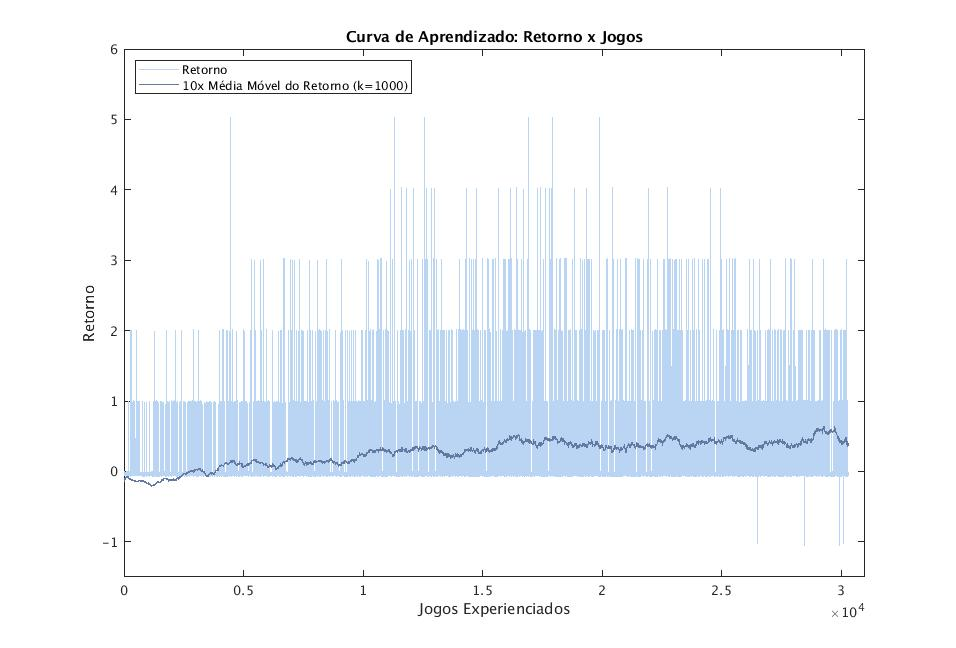
\includegraphics[width=1\linewidth]{figs/curva-sarsa-1.jpg}
	\centering
	\caption{Curva de aprendizado do agente com comportamentos pré-programados utilizando Sarsa aproximado.}
	\label{fig:single-agent-sarsa-behaviors}
\end{figure}

\section{\textit{Q-Learning} Duplo Tabular e Comportamentos Pré-Programados}
\label{sec:behaviors-tabular}

Para este experimento, o aproximador de função foi substituído por uma tabela e o algoritmo Sarsa pelo Q-Learning. Foram executados 3 treinamentos de 100.000 episódios e a tabela Q completa e o histórico dos retornos obtidos pelo agente ao longo do treinamento foram salvos.

O gráfico da Figura \ref{fig:single-agent-tabular-behaviors} mostra o histórico médio dos 3 treinamentos.
Observa-se que há uma estagnação do retorno por volta das 60.000 amostras, o que pode indicar a necessidade de ajuste no decaimento do fator de exploração para que o agente explore novas possibilidades por mais episódios. Isso mostra a importância de buscar equilíbrio no dilema da exploração e aproveitamento, discutido na Seção \ref{subsec:exploration-exploitation}.

A estagnação pode indicar, também, existência de um limite superior para o desempenho do agente devido à menor flexibilidade da política aprendida, ou seja, o agente só é capaz de construir a política a partir dos comportamentos pré-programados.

\begin{figure}[H]
	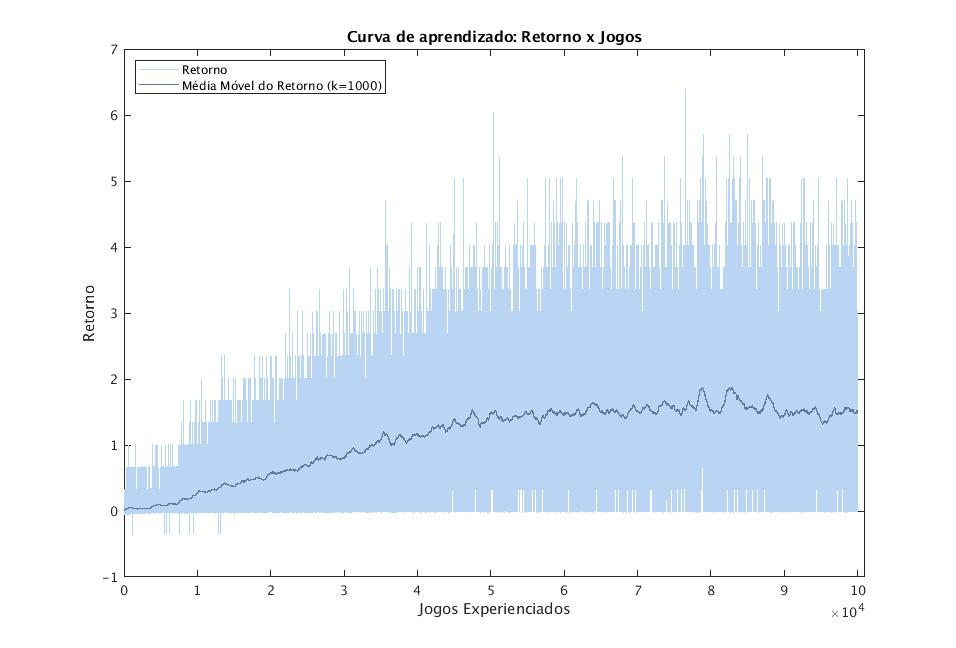
\includegraphics[width=0.95\linewidth]{figs/curva-behaviors-tabular.jpg}
	\centering
	\caption{Curva de aprendizado do agente com comportamentos pré-programados.}
	\label{fig:single-agent-tabular-behaviors}
\end{figure}

A Figura \ref{fig:goal-seq} ilustra o agente único treinado conduzindo a bola e realizando um gol conforme a política aprendida.

\begin{figure}[H]
	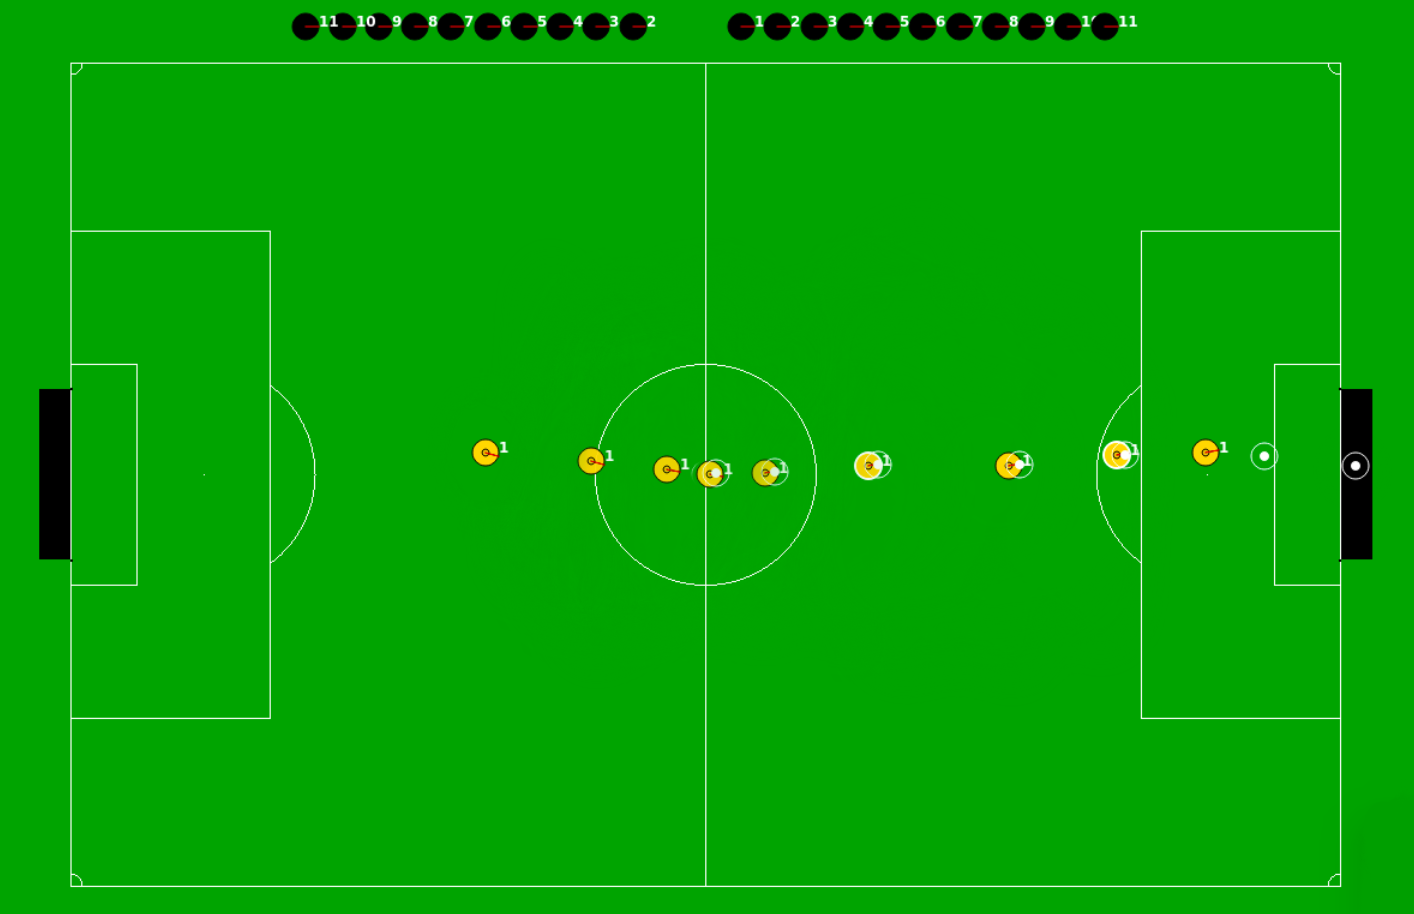
\includegraphics[width=0.9\linewidth]{figs/goal-sequence.png}
	\centering
	\caption{Sobreposição de sequência de imagens do agente único fazendo gol.}
	\label{fig:goal-seq}
\end{figure}

A Figura \ref{fig:curvalonga-bhv} mostra o histórico de retornos para um treinamento mais longo, de 200.000 episódios. Nela percebe-se que, após a cessação da exploração, o agente estabiliza seu desempenho um pouco abaixo do máximo obtido.

\begin{figure}[H]
	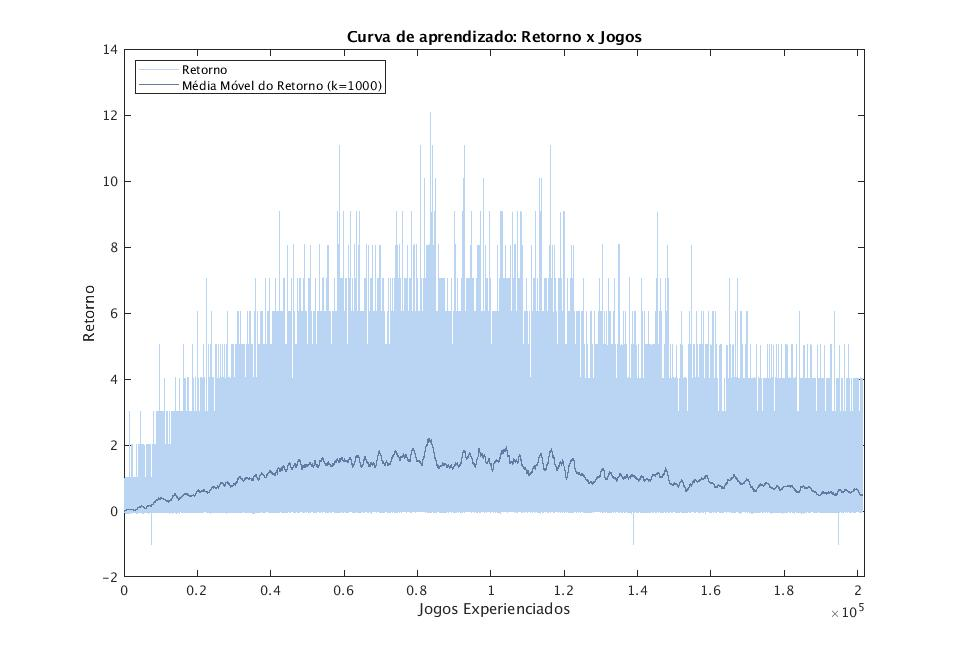
\includegraphics[width=1\linewidth]{figs/curvalonga-behaviors-tabular.jpg}
	\centering
	\caption{Curva de aprendizado do agente com comportamentos pré-programados para treinamento longo.}
	\label{fig:curvalonga-bhv}
\end{figure}

Utilizando os pesos obtidos em uma das execuções do treinamento é possível observar cenários variados da política aprendida com um único agente e a bola em campo. A Figura \ref{fig:behaviors-result} ilustra quatro situações distintas construídas com sobreposição de imagens a cada 50 ciclos. Em três delas, o agente marcou um gol em tempos variados, ora tocando a bola até a área do gol, ora chutando de uma distância maior. A quarta situação, no canto inferior direito, ilustra uma situação em que o agente não realizou gols e ficou parado após tocar a bola para trás.

\begin{figure}[H]
	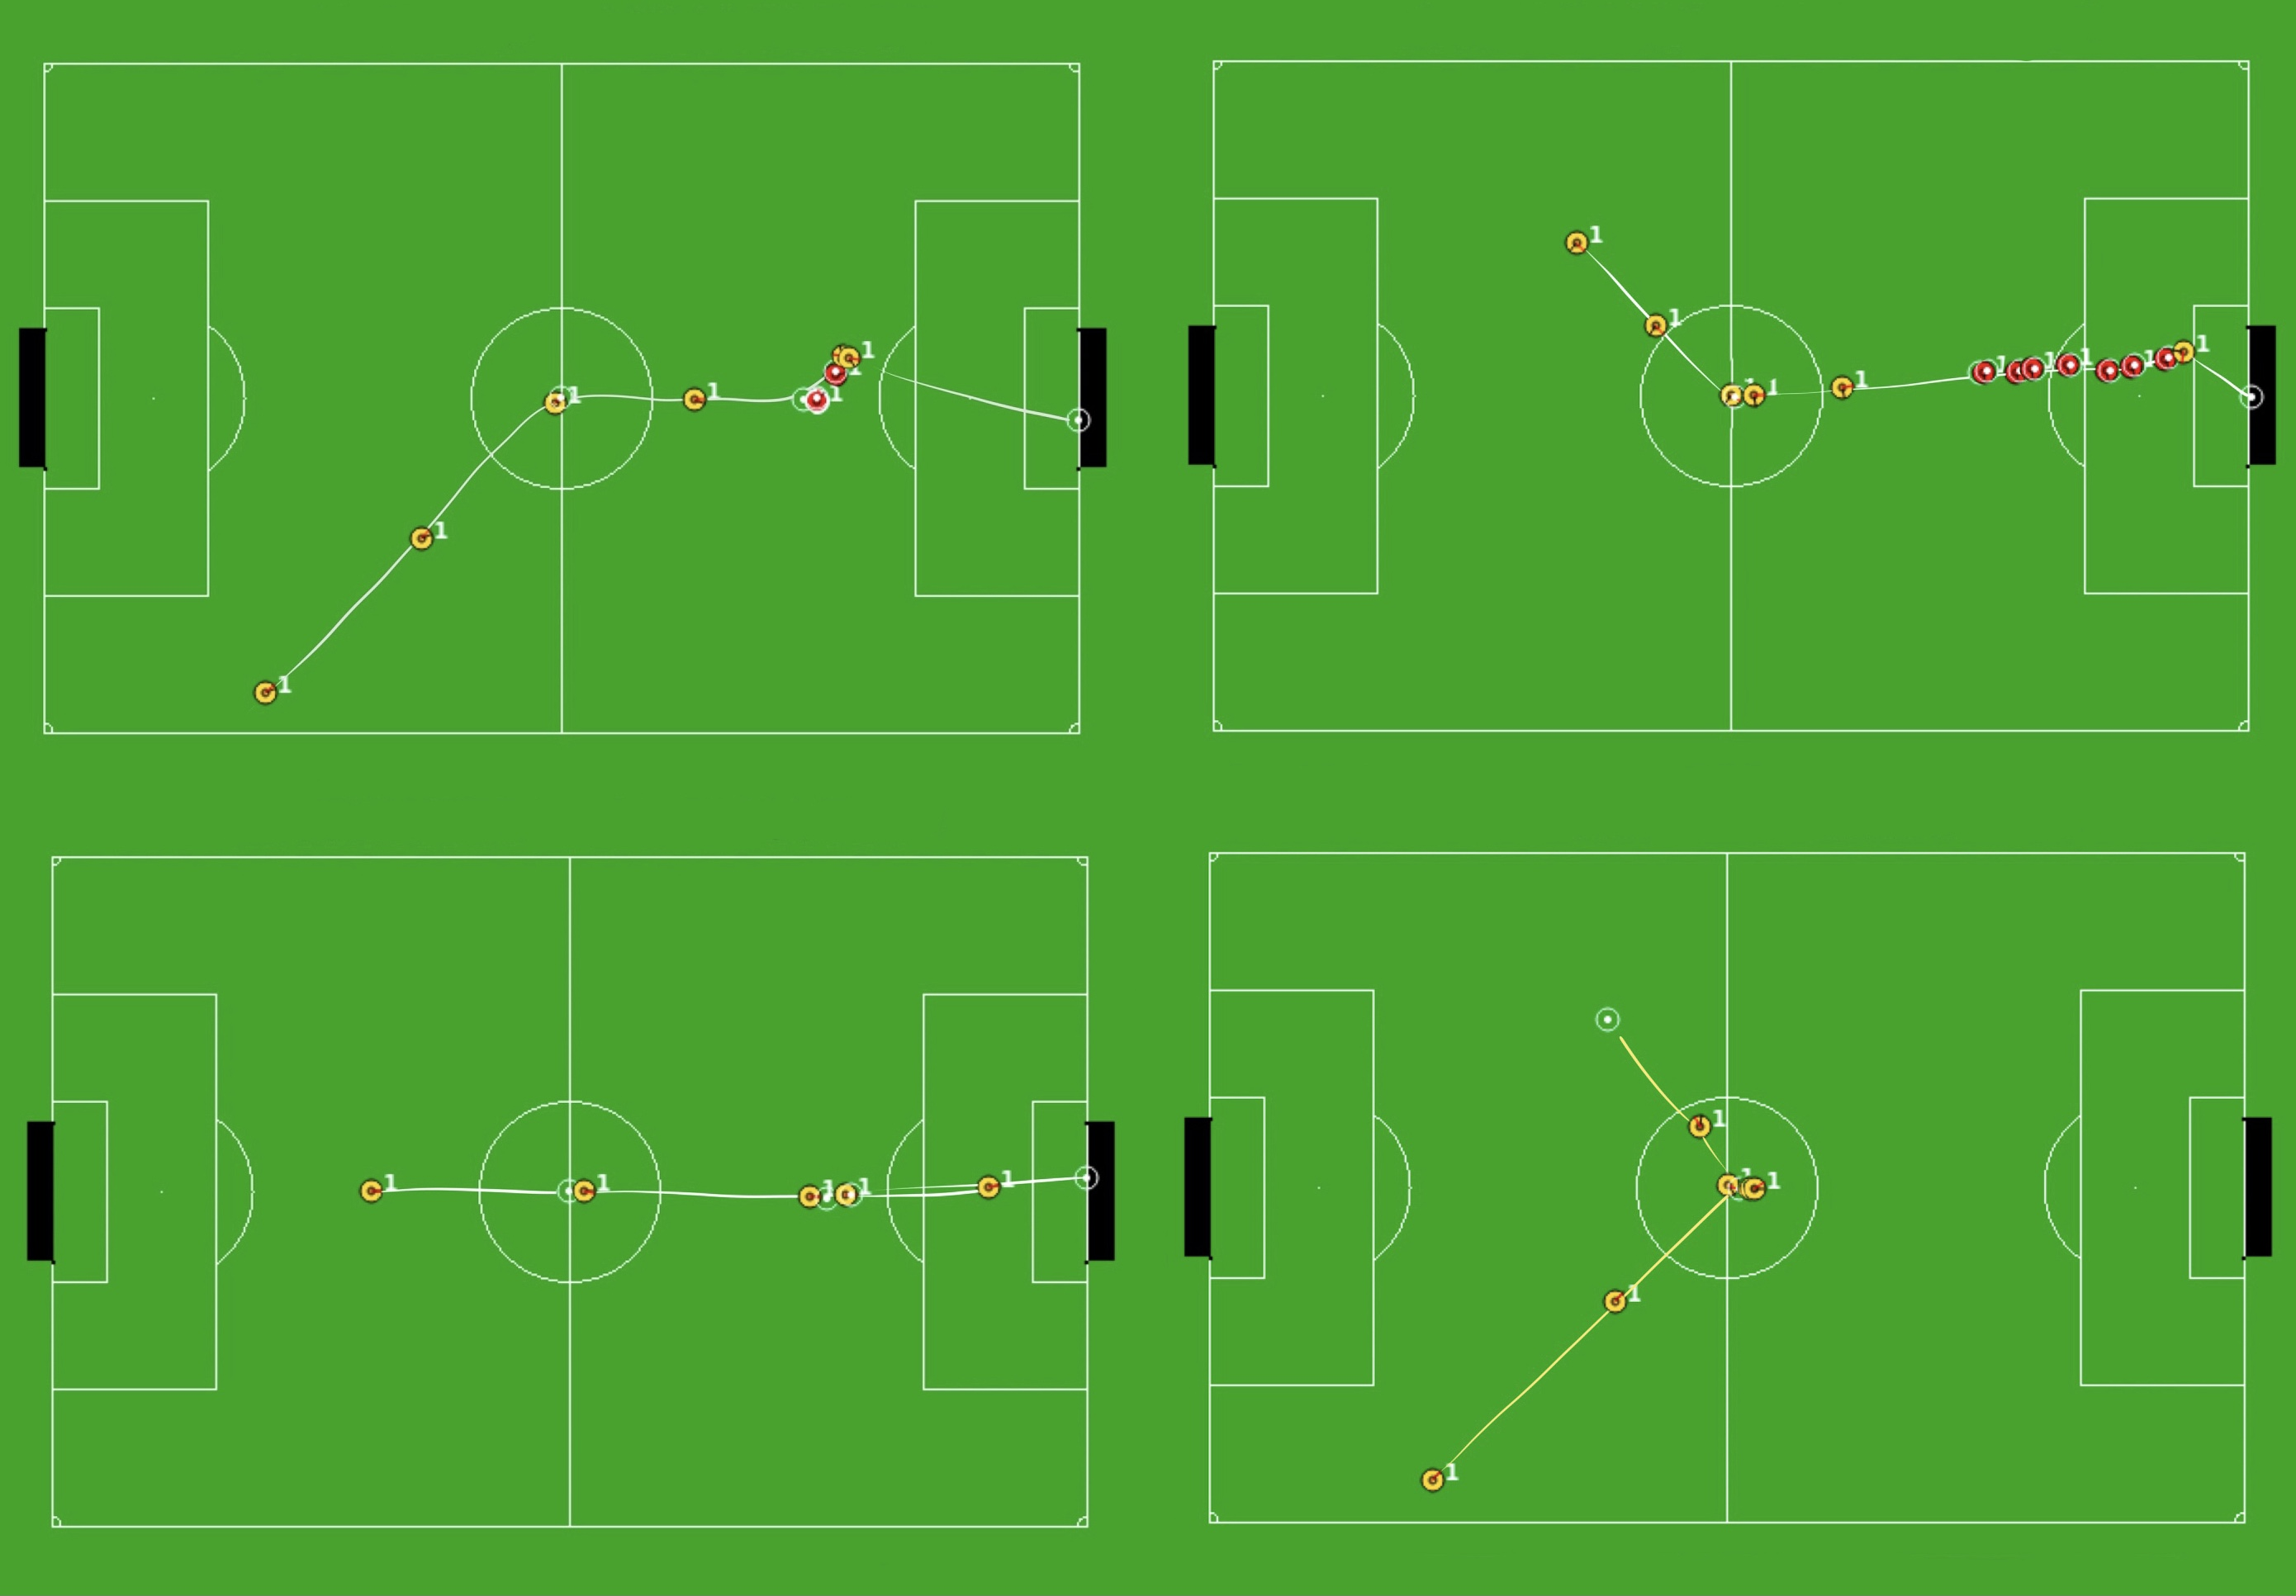
\includegraphics[width=1\linewidth]{figs/behaviors-result.jpg}
	\centering
	\caption{Montagem ilustrando 4 exemplos da política aprendida através de sobreposição de imagens.}
	\label{fig:behaviors-result}
\end{figure}


\section{\textit{Q-Learning} Duplo Tabular e Ações Elementares}

Substituindo os comportamentos pré-programados por uma seleção de ações elementares, foram executados 3 treinamentos distintos de 100.000 treinamentos de  partidas a fim de suavizar o elemento sorte nos resultados. Após cada um dos treinamentos, foram salvos a tabela Q completa e o histórico dos retornos obtidos pelo agente ao longo do treinamento.

A Figura \ref{fig:single-agent-curva} mostra esse histórico. É interessante observar que, com o decaimento dos fatores de exploração e de aprendizagem, após 100.000 episódios, ambos eram $\epsilon \approx 0.074074$ e $\alpha \approx 0.056604$, ou seja, o agente já executava na maior parte dos ciclos a política aprendida. Para cada jogo foi feita a média entre os 3 retornos observados em cada um dos treinamentos.

\begin{figure}[H]
	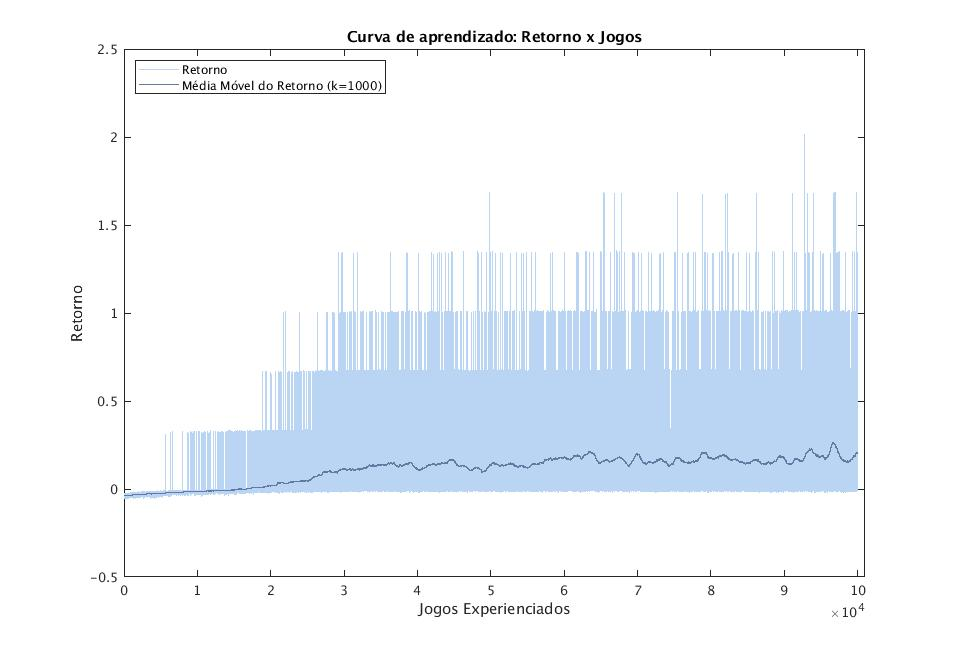
\includegraphics[width=0.93\linewidth]{figs/curva-qtabular.jpg}
	\centering
	\caption{Curva de aprendizado do agente com ações elementares. }
	\label{fig:single-agent-curva}
\end{figure}

\begin{figure}[H]
	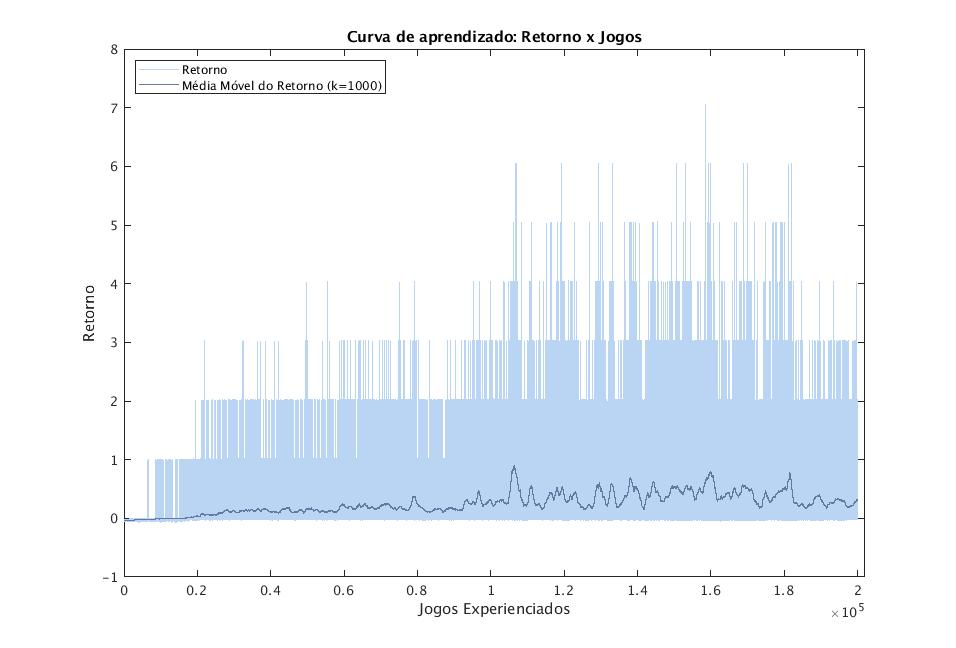
\includegraphics[width=0.93\linewidth]{figs/curvalonga-qtabular.jpg}
	\centering
	\caption{Curva de aprendizado para treinamento longo.}
	\label{fig:single-agent-curvalonga}
\end{figure}

Além disso, assim como na Seção \ref{sec:behaviors-tabular}, foi executado um treinamento de 200.000 episódios a fim de observar a aprendizagem por um período mais longo. Na Figura \ref{fig:single-agent-curvalonga}, observa-se que o agente continua melhorando seu desempenho até próximo do fim do treinamento, o que pode ser indício de que o aprendizado com ações elementares de fato permite mais flexibilidade na política aprendida.

Apesar da grande quantidade de experiência a que o agente teve acesso, nota-se na Figura \ref{fig:single-agent-curvalonga} que o crescimento de seu desempenho é bastante limitado, sequer atingindo a média de 1 gol por episódio. Isso é um indicativo do altíssimo custo computacional de soluções utilizando ações elementares como a utilizada no experimento, especialmente quando o espaço de estados é vasto.

O capítulo seguinte relata as conclusões acerca desse trabalho, sua contribuição para a área e discorre sobre possíveis trabalhos para continuação do desenvolvimento da plataforma, especialmente dentro do contexto da Universidade de Brasília.

% \section{Agentes Concorrentes}

% Após validação do sistema com agente único, é interessante experimentar com treinamento adversarial de apenas 2 jogadores em formato um-contra-um. A intenção dessa etapa é experimentar com o sistema o caso adversarial, no qual há um ou mais agentes com objetivo oposto ao do agente sendo treinado.
 
% \section{Múltiplos Agentes}

% Após validar os casos de agente único e de agentes concorrentes, propõe-se um treinamento completo em jogos 11 contra 11. O objetivo é, ao final do processo, termos um time capaz de jogar contra os principais times da atualidade na categoria RoboCup Soccer Simulation 2D.

% Para isso, os agentes devem ser capazes de cooperar e reagir aos movimentos da equipe oposta a fim de marcar gols e evitar os gols do adversário.
